\documentclass[a4paper]{article}

\usepackage{url}
\usepackage{graphicx}	% For figure environment
\usepackage{epstopdf}
\usepackage[center]{subfigure}
\usepackage{amssymb}	% For mathematical figures like \mathbb{R}
\usepackage{amsmath}
\usepackage{framed}
\usepackage{tikz}
\usetikzlibrary{mindmap,trees}
\usepackage{pdflscape}
\usepackage[a4paper]{geometry}
\usepackage{subfiles}


\title{Advanced Systems Lab - Milestone I} 
\author{Lukas Elmer, Matthias Ganz} 
\date{\today} 


\begin{document}

\maketitle


\begin{abstract}

This document, describes the message queuing system which was build. Architecture and design choices are shown and explained. Further test scenarios and test loads are defined. Resulting test output is described and analysed.

\end{abstract}

%% %%%%%%%%%%%%%%%%%%%%%%%%%%%%%%%%%%%%%%%%%%%%%%
\section{Messaging System}
In this section the system under test (also named as middle ware component) is described.


%% ----------------------------------------------
\subsection{Overview}

Figure \ref{fig:system-overview} shows a generic setup of the messaging system. Multiple middle ware components are connected to a single database and severs a couple of clients. Application state is persisted on the database, therefore a middle ware component can be considered as stateless.

% ------------------------------------------------
% Figure - system overview

\begin{figure}
  \begin{center}
    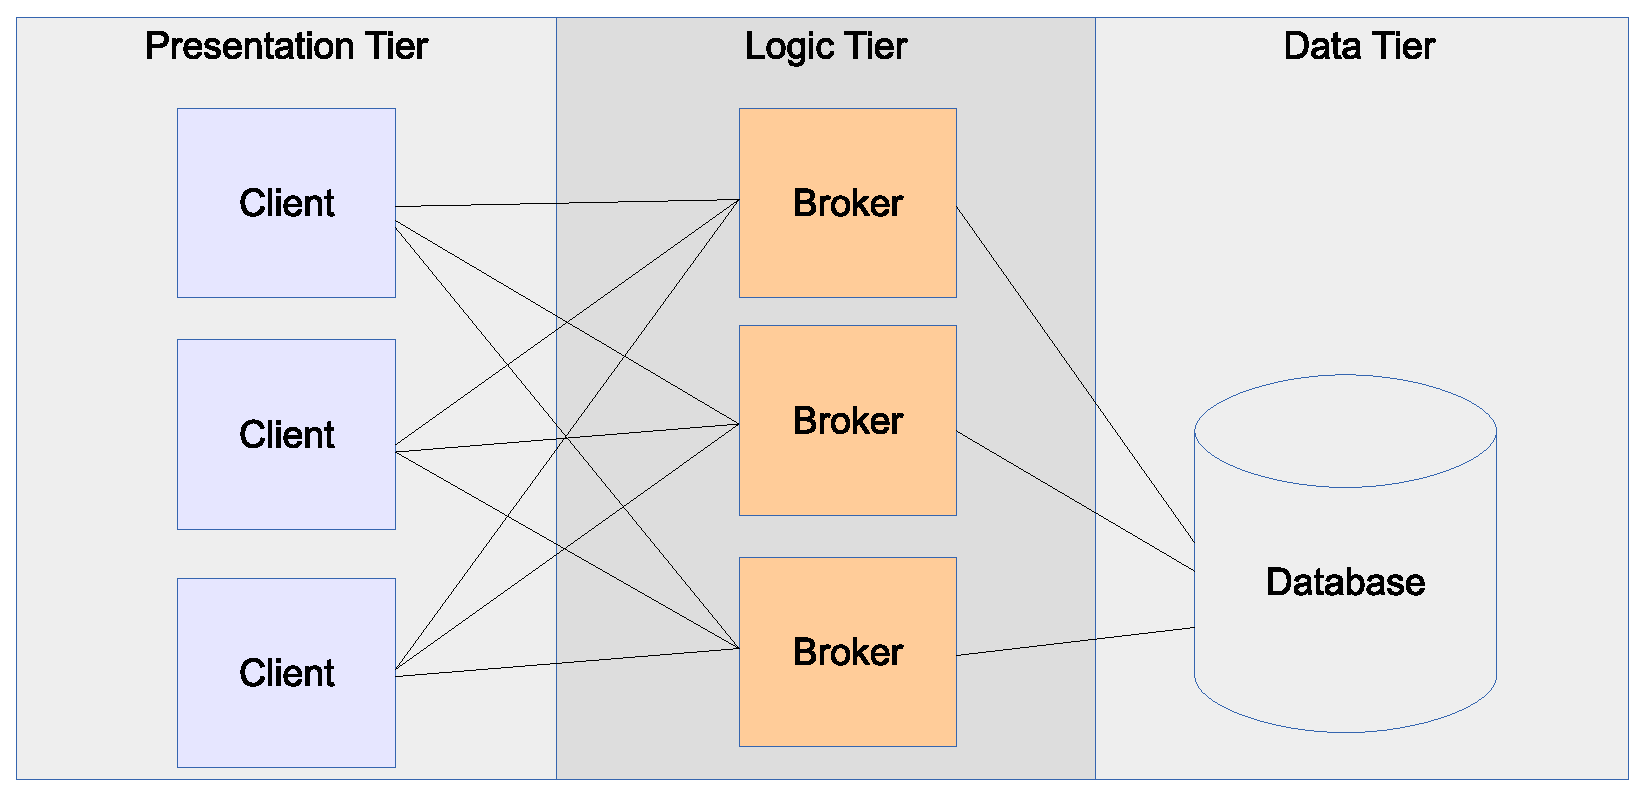
\includegraphics[scale=0.4]{../drawings/system-overview.eps}
  \end{center}
  \caption{System Overview}
  \label{fig:system-overview}
\end{figure}

Figure \ref{fig:middleware-threading} shows important software components of a single middle ware. A nonblocking network interface (NIO) handles communication to the clients. Received data is put to a single thread safe request queue.

A configurable number of workers are constantly reading from the request queue. As soon as a worker gets a piece of work (request raw data) it then performs the following tasks:
\begin{itemize}
\item decoding: The raw request is parsed and converted into a request java object
\item process: The request is processes. The database is accesses and a response object is created
\item encode: The response object is serialized and placed into the response queue of the network interface.
\end{itemize}

% ------------------------------------------------
% Figure - threading

\begin{figure}
	\begin{center}
    \includegraphics[scale=0.4]{../drawings/broker-threading.eps}
  \end{center}
  \caption{Middleware's main Components}
  \label{fig:middleware-threading}
\end{figure}

%% ----------------------------------------------
% Section Design Decisions
%% ----------------------------------------------
\subfile{part02-design.tex}


%% ----------------------------------------------
% Section Performance Relevant Features
%% ----------------------------------------------
\subfile{part03-features.tex}

%% ----------------------------------------------
% Section Experiments
%% ----------------------------------------------
\subfile{part04-experiments.tex}

\section{References}

% TODO

http://dl.acm.org/citation.cfm?id=SERIES12798.1557393

@book{hanmer2007patterns,
  title={Patterns for fault tolerant software},
  author={Hanmer, Robert},
  year={2007},
  isbn = {0470319798, 9780470319796},
  publisher={Wiley Publishing}
}

%\bibliography{mybib}

%% %%%%%%%%%%%%%%%%%%%%%%%%%%%%%%%%%%%%%%%%%%%%%%%%%%%%%%%%%%%%%%%%%%%%%%%%%
\section{Notes - to delete}

\subsection{What should be included in this report }

\subsubsection{System Code}
\begin{itemize}
\item Code
\item Scripts for experiment
\end{itemize}

\subsubsection{Experimental data}
\begin{itemize}
\item Basic tests ans simple traces
\item Long running traces, Raw data and graphs for all experiments
\end{itemize}

\subsubsection{Written report}
\begin{itemize}
\item Architectural  diagrams
\item Interface description
\item explanation of the system design
\item Description of all experiments
\item statistical treatment of data
\item commentary analysis
\end{itemize}


\end{document}
